Paātrinātāja sistēma realizēta VHDL un novērtēta ar reprezentatīviem dziļajiem konvolucionālajiem impulsu neironu tīkliem.
Realizācija sintezēta, izvietota un trasēta ar \textit{AMD Vivado} rīku \textit{Xilinx Kintex UltraScale KU115-2}
\Gls{fpga} iekārtai. Turpmākajās sadaļās norādītais resursu izmantojums, maksimālā darbības frekvence, latentums un jaudas patēriņš
iegūti realizētajam projektam.

Eksperimentālā pārbaude veikta ar \textit{Alpha Data ADM-PCIE-8K5}\footnote{https://alpha-data.com/product/adm-pcie-8k5/}
PCIe paātrinātāja karti, kurā izmantots \textit{Kintex UltraScale KU115-2} \Gls{fpga}. \Gls{fpga} karte uzstādīta
\textit{NVIDIA Jetson AGX Orin}\footnote{https://www.nvidia.com/en-us/autonomous-machines/embedded-systems/jetson-orin/}
iegultajā skaitļošanas platformā, kas kalpo par procesoru un atbild par tīkla konfigurāciju, datu
pārsūtīšanu un rezultātu savākšanu. Saziņa starp to un paātrinātāju notiek pa PCI Express saskarni, savukārt
\Gls{fpga} pēc nepieciešamo konfigurācijas parametru un ieejas impulsu straumju saņemšanas izpilda uz notikumiem balstīto
apstrādi. Eksperimentālā platforma parādīta \ref{fig:fpga_jetson}. attēlā.
\begin{figure}[!t]
\centering
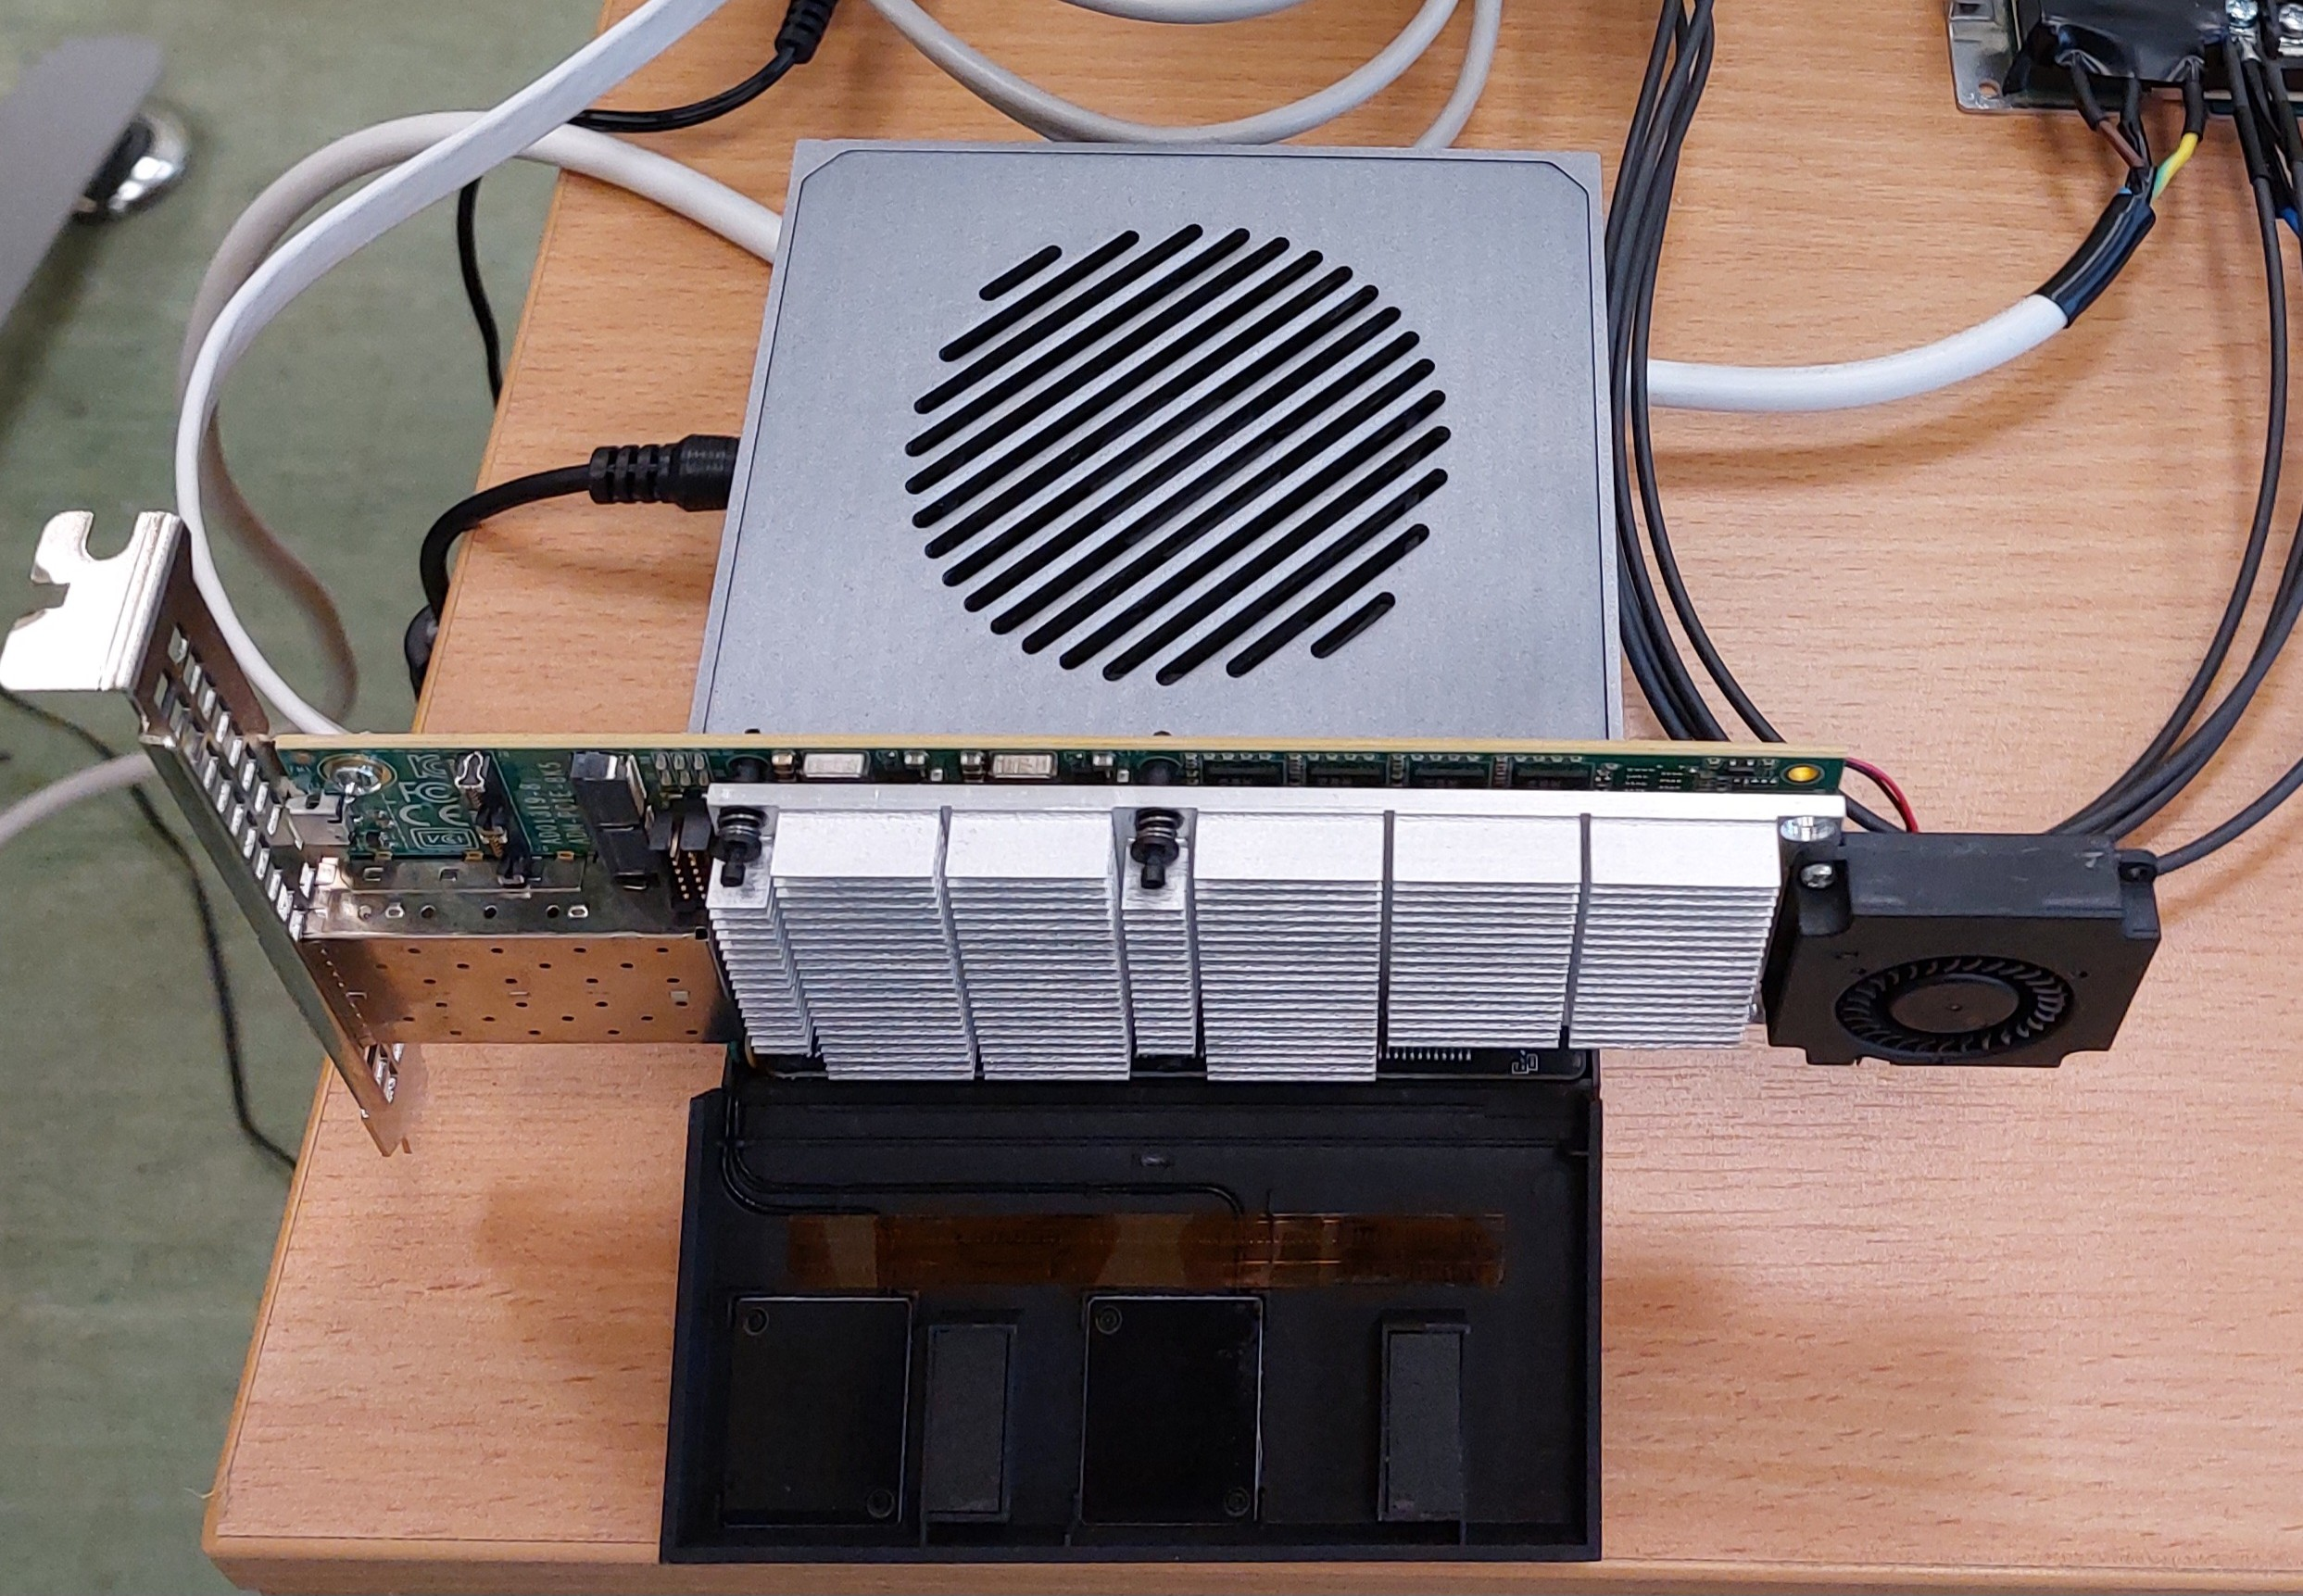
\includegraphics[width=0.8\linewidth]{fig/fpga_jetson.jpg}
\caption{Eksperimentālā novērtējuma platforma, kas sastāv no \textit{NVIDIA Jetson AGX Orin} sistēmas un \textit{Alpha Data ADM-PCIE-8K5} PCIe FPGA paātrinātāja kartes.}
\label{fig:fpga_jetson}
\end{figure}

Tādējādi platforma apvieno procesorā darbināmas programmatūras elastību ar \Gls{fpga} aparatūras uz notikumiem balstītu izpildi, nodrošinot vidi perifērijas mākslīgā intelekta lietojumiem paredzētu neiromorfo paātrinātāju pētniecībai.

Šī platforma ļauj realizēt \ref{fig:overall_arch}. attēlā parādīto straumēšanas paātrinātāju. Straumēšanas paātrinātājs
aprīkots ar AXI Stream saderīgām saskarnēm, savukārt PCIe \Gls{dma} modulis pārsūta konfigurāciju un datus starp
procesoru un \Gls{fpga} ierīci. Iegultajā sistēmā nodrošinātas programmatūras abstrakcijas kvantētu \Gls{snn} modeļu ielādei un
efektīvai impulsu datu apmaiņai \Gls{aer} reprezentācijā. Modeļa parametri, tostarp kvantētie konvolūcijas svari un nobīdes,
kā arī neironu slāņu konfigurācijas vērtības (solis, malu papildinājums, sliekšņi, laika konstantes), tiek pārsūtīti
paātrinātājam, izmantojot atmiņā kartētu piekļuvi pa PCIe saskarni. Šie parametri tiek ierakstīti mikroshēmas iekšējos
konfigurācijas reģistros un BRAM ar AXI-Lite transakcijām. Izpildes laikā laikā kodētās impulsu straumes starp procesoru
un paātrinātāju tiek apmainītas kā \Gls{aer} paketes \Gls{dma} straumēs. Šis ļauj ieviest kvantētus dziļos
\Gls{snn} modeļus un atvieglo integrāciju ar augstāka līmeņa ietvariem, piemēram, \textit{PyTorch} un \textit{SpikingJelly}.


